\documentclass[12pt]{article}

%%%%%%%%%%%%%%%%% common packages are included here %%%%%%%%%%%%%%%%%
%\usepackage[pdftex,draft]{graphicx}
\usepackage[pdftex]{graphicx}
\usepackage[pdftex]{hyperref}
\usepackage{epstopdf}
\usepackage{tabularx}
\usepackage[lofdepth,lotdepth]{subfig} % subfloat
\usepackage{bm} % bold math
\usepackage{color}
\usepackage[centertags]{amsmath}
\usepackage{mathrsfs}
\usepackage{amsmath}
\usepackage{mathtools}
\usepackage{amssymb}
\usepackage{amsfonts}
\usepackage{amsthm}
\usepackage{newlfont}
\usepackage{textcomp,gensymb} % for \textcelsius, \textdegree, and \degree
\usepackage{syntonly}
\usepackage[toc,page]{appendix}
\usepackage{setspace}
\usepackage[export]{adjustbox}
\usepackage[percent]{overpic}
\usepackage{booktabs}
\usepackage{cite}
\usepackage{notoccite}

%%%%%%%%%%%%%%%%%%%% some declaration %%%%%%%%%%%%%%%%%%%%%
\DeclareGraphicsExtensions{.pdf,.PDF,.png,.PNG,.jpg,.eps}
%\graphicspath{{./figures/}}
\onehalfspacing
%\doublespacing
\setcounter{secnumdepth}{3}

%%%%%%%%%%%%%%%%%%% new commands are defined here %%%%%%%%%%%%%%%%%%%%%
\newcommand{\dg}{$^{\circ}$} % degree symbol
\newcommand{\iang}{\AA$^{-1}$} % inverse Angstrom symbol
\newcommand{\degC}{$^{\circ}\mathrm{C}$} % degree Celcius
\newcommand{\Eq}[1]{Eq.\,(\ref{#1})} % reference to an equation

% Some mathematical (physical) quantities and symbols that are used often
\newcommand{\xhat}{\mathbf{\hat{x}}}
\newcommand{\yhat}{\mathbf{\hat{y}}}
\newcommand{\zhat}{\mathbf{\hat{z}}}
\newcommand{\kin}{\mathbf{k}_{\mathrm{in}}}
\newcommand{\kout}{\mathbf{k}_{\mathrm{out}}}
\newcommand{\Tat}{\mathrm{Tat}}
\newcommand{\DOPC}{\mathrm{DOPC}}
\newcommand{\cm}{\mathrm{cm}}
\newcommand{\dx}{\mathop{dx}}
\newcommand{\dy}{\mathop{dy}}
\newcommand{\dz}{\mathop{dz}}
\newcommand{\dr}{\mathop{dr}}

% To simplify some formatting issues
\newcommand{\pars}[1]{\mathopen{}\left( #1 \right)\mathclose{}} % () without extra spaces due to \left and \right
\newcommand{\bracks}[1]{\mathopen{}\left[ #1 \right]\mathclose{}} % [] without extra spaces
\newcommand{\angles}[1]{\mathopen{}\left\lange #1 \right\rangle\mathclose{}} % <> without extra spaces
\newcommand{\braces}[1]{\mathopen{}\left\lbrace #1 \right\rbrace\mathclose{}} % {} without extra spaces
\newcommand{\ds}[1]{\displaystyle{#1}}%
\newcommand{\+}{^{\dagger}}%                                
\newcommand{\partiald}[3][]{{\partial^{#1}#2 \over \partial {#3}^{#1}}}%

% Hyphenation
\hyphenation{multi-lamellar}
\hyphenation{table}

\topmargin -0.3in
\oddsidemargin 0.5in
\evensidemargin 0.5in
\textheight 8.5in
\textwidth 6.0in

\date{\today}

\begin{document}
\section{Thin Rod Model of the ripple phase}
The thin rod model will be applied to the ripple phase WAXS. 
In this model, electron density of lipid chains are described as delta 
functions and lipid head groups are assumed not to contribute to scattering. 
Since the molecular packing of the major side of ripple phase is hypothesized 
to be gel-like, the model may be adequate. First, we will study diffraction 
from chains packed in gel phase manner whose system size is infinite but whose 
packing plane make an angle $\xi$ with the $xy$ plane. 
This infinite case is adequate for indexing the ripple Bragg peaks while
it ignores the peak broadening effect.
The system will later be truncated along the ripple direction to see the effect 
of the finite size on peak broadening. Finally, in-plane powder will be taken 
into account to derive a peak intensity pattern.

First, let us calculate the positions of the diffraction peaks from a two 
dimensional orthorhombic lattice whose plane makes an angle $\xi$ with 
respect to the $xy$ plane and extends to infinity. 
As a unit cell, we will take a parallelpipedon containing two rods,
one located at the origin and the other located at the center
(Fig.~\ref{fig:unit_cell_waxs}).
The lattice vectors are $\mathbf{a_1}=a_1\cos\xi\xhat+a_1\sin\xi\zhat$ 
and $\mathbf{a_2}=a_2\yhat$. \textcolor{red}{There are other choices for
how the lattice is oriented with respect to the ripple direction,
which should be considered as well.}
Then, the Laue conditions are given by
\begin{align}
	2\pi h &=\mathbf{q}\cdot\mathbf{a_1}=(a_1\cos\xi)q_x+(a_1\sin\xi)q_z \\
	2\pi k &=\mathbf{q}\cdot\mathbf{a_2}=a_2 q_y,
\end{align}
with $h$ and $k$ being zero or integer. 
Let us define the chain tilt angle $\theta$ to be the angle between
the stacking $z$ direction and the chain direction. We also define
$\phi$ to represent the direction into which chains are tilted.
In other words, $\theta$ and $\phi$ are usual spherical coordinates
with respect to the ripple $x$, $y$, and $z$ axes, not the local
bilayer Cartesian axes. With this choice of coordinates, chains 
are tilted with respect to the local bilayer normal if 
$\theta$ = 0. $\theta=\xi$ and $\phi=\pi$ gives chains parallel to the
local bilayer normal, or $\theta_t$ = 0. 
\textcolor{red}{It would be good to work out
the relation between $\theta$ and $\theta_t$, $\theta_t$ being the chain tilt
with respect to the local bilayer normal.}

\begin{figure}
  \centering
  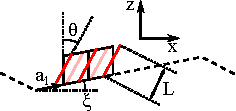
\includegraphics[width=0.8\textwidth]{unit_cell_waxs_side} \\
  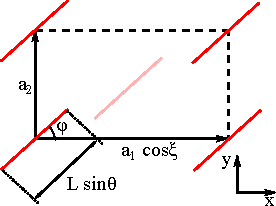
\includegraphics[width=0.6\textwidth]{unit_cell_waxs_top}
  \caption[Unit cell for chain packing in the major arm]
  {Unit cell for chain packing in the major arm. 
  (top) Projection of the unit cell in the $xz$-plane. The unit cell is taken
  as a parallelpipedon shown by black solid lines, each unit cell 
  containing two chains.
  Chains located at the center of the unit cell are
  drawn as opaque red lines while chains at the lattice points are 
  drawn as solid red lines. The dash line indicates
  the mid-plane of a rippling bilayer. Chains are tilted with respect to
  the stacking $z$ direction by $\theta$ and the major arm is tilted 
  with respect to the ripple $x$ direction by $\xi$. The chain length
  is denoted by $L$. $\mathbf{a_1}$ and $\mathbf{a_2}$ are orthorhombic 
  unit cell vectors.
  (bottom) Projection of the unit cell in the $xy$-plane.
  $\phi=0$ means chains are tilted in the $xz$ plane and $\phi=\pi/2$
  means chains are titled into the direction perpendicular to the 
  ripple direction.}
  \label{fig:unit_cell_waxs}
\end{figure}

The electron density, assuming a delta function for each chain, is given by 
\begin{align}
	\rho(\mathbf{r})&=\delta(x-\alpha z, y-\beta z)+\\
	&\delta\left[x-\frac{a_1\cos\xi}{2}-\alpha\left(z-\frac{a_1\sin\xi}{2}\right),\, y-\frac{a_2}{2}-\beta\left(z-\frac{a_1\sin\xi}{2}\right)\right],
\end{align}
where $\alpha=\tan\theta\cos\phi$ and $\beta=\tan\theta\sin\phi$. The first rod extends for
\begin{align}%Range of extension of first rod
	-L/2\sin\theta\cos\phi\leq &x\leq L/2\sin\theta\cos\phi\\ 
	-L/2\sin\theta\sin\phi\leq &y \leq L/2\sin\theta\sin\phi\\
	-L/2\cos\theta\leq &z \leq L/2\cos\theta,
\end{align}
and the second rod for
\begin{align}%Range of extension of second rod
	-L/2\sin\theta\cos\phi+a_1/2\cos\xi\leq &x\leq L/2\sin\theta\cos\phi+a_1/2\cos\xi\\ 
	-L/2\sin\theta\sin\phi+a_2/2 \leq &y \leq L/2\sin\theta\sin\phi+a_2/2\\
	-L/2\cos\theta+a_1/2\sin\xi \leq &z \leq L/2\cos\theta+a_1/2\sin\xi.
\end{align}
Then, the form factor is given by
\begin{align}%form factor calculation
	F(\mathbf{q})&=\int dx\int dy\int dz\,\rho(\mathbf{r})\,e^{i\mathbf{q}\cdot\mathbf{r}}\\
	&=\int_{-\frac{L}{2}\cos\theta}^{\frac{L}{2}\sin\theta}dz e^{i(\alpha q_x+\beta q_y+q_z)z}\,+\nonumber\\
	&\int_{-\frac{L}{2}\cos\theta+\frac{a_1}{2}\sin\xi}^{\frac{L}{2}\cos\theta+\frac{a_1}{2}\sin\xi}dz\, e^{\frac{i}{2}\left[q_x\left(a_1\cos\xi-\alpha a_1\sin\xi\right)+q_y\left(a_2-\beta a_1\sin\xi\right)\right]}\,e^{i(\alpha q_x+\beta q_y+q_z)z}\nonumber\\
	&=\left[1+e^{\frac{i}{2}\left(a_1\cos\xi q_x+a_1\sin\xi q_z+a_2q_y\right)}\right]\frac{2}{\gamma}\sin\left(\frac{\gamma L\cos\theta}{2}\right)\nonumber\\
	&=\left[1+e^{i\pi(h+k)}\right]\frac{2}{\gamma}\sin\left(\frac{\gamma L\cos\theta}{2}\right)\label{eq:FormFactor},
\end{align}
where $\gamma=\alpha q_x+\beta q_y+q_z$. Eq. \ref{eq:FormFactor} shows that peaks with $h+k$ being odd is extinct. For $h+k$ even, we have
\begin{equation}%form factor for even h+k
	F(\mathrm{q})=\frac{4}{\gamma}\sin\left(\frac{\gamma L\cos\theta}{2}\right)\label{eq:FormFactorEven}.
\end{equation} 

For (20) peak, $q_y$ = 0 and $4\pi=a_1\cos\xi q_x+a_1\sin\xi q_z$. The second equation can be rewritten to give
\begin{equation}
	q_z=-\frac{1}{\tan\xi}q_x+\frac{4\pi}{a_1\sin\xi}
\end{equation}
which defines a straight line in $q_xq_z$-plane along which (20) Bragg rod appears. Eq. \ref{eq:FormFactorEven} has a peak at $\gamma$ = 0. Hence, the maximum intensity of (20) peak is at $q_x$ and $q_z$ that satisfy Laue conditions and $\gamma$ = 0. This gives three equations and three unknowns. Explicitly written, we have
\begin{align}
	q_y &= 0\\
	4\pi &= a_1\cos\xi q_x+a_1\sin\xi q_z\\
	0 &= \tan\theta\cos\phi q_x+q_z
\end{align}
Solving these, we get
\begin{align}%q_x and q_z equations for (20) peak
	q_x &= \frac{4\pi}{a_1\cos\xi(1-\tan\theta_t\cos\phi\tan\xi)}\\
	q_z &= \frac{-4\pi\tan\theta_t\cos\phi}{a_1\cos\xi(1-\tan\theta_t\cos\phi\tan\xi)}
\end{align}
For $\phi$ = $\pi$/2, we have $q_x=4\pi/(a_1\cos\xi)$ and $q_z=0$, so one would expect to see a peak on the equator, the case of which is similar to $L_{\beta I}$ phase in gel phase. To get back to ordinary gel phase, $\xi$ should be set equal to zero.

For any (hk) line, we again have three equations and three unknowns as
\begin{align}
	2\pi h &= q_xa_1\cos\xi +q_za_1\sin\xi\\
	2\pi k &= q_ya_2\\
	0 &= q_x\tan\theta_t\cos\phi + \frac{2\pi k}{a_2}\tan\theta_t\sin\phi +q_z
\end{align}
Solving for $q_x$, $q_y$, and $q_z$, we obtain
\begin{align}
	q_x &= \frac{2\pi(h+ka\beta\sin\xi)}{a_1\cos\xi(1-\alpha\tan\xi)}\\
	q_y &= \frac{2\pi k}{a_2}\\
	q_z &= \frac{-2\pi(h\alpha+ka\beta\cos\xi)}{a_1\cos\xi(1-\alpha\tan\xi)},
\end{align}
where $a=a_1/a_2$.

\end{document}